%-*-latex-*-
\sectionthree{Fake root heap}
\begin{python0}
from solutions import *; clear()
\end{python0}

Suppose you have two max heaps.
One quick way to merge them is to simply create a new root
and join the new root to the two roots as parent.
The value of the new root can be any arbitrary value that
is larger than the values of the two roots.
To remind myself that the new root is not really a value in the
heap, I can use a flag in each node.
Another thing that I can do it to use a value that is sentinel.
In the case of max heap, say I call this value $\infty$.

For instance say you have these two max heaps:
\begin{center}
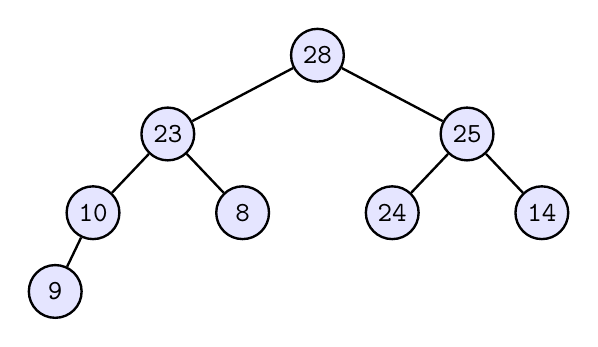
\begin{tikzpicture}

\fill[blue!10] (0.0, 0.0) circle (0.35);
\node [line width=0.03cm,black,minimum size=0.6699999999999999cm,draw,circle] at (0.0,0.0)(28){};\draw (0.0, 0.0) node[color=black] {\texttt{28}};
\fill[blue!10] (-1.9, -1.0) circle (0.35);
\node [line width=0.03cm,black,minimum size=0.6699999999999999cm,draw,circle] at (-1.9,-1.0)(23){};\draw (-1.9, -1.0) node[color=black] {\texttt{23}};
\fill[blue!10] (1.9, -1.0) circle (0.35);
\node [line width=0.03cm,black,minimum size=0.6699999999999999cm,draw,circle] at (1.9,-1.0)(25){};\draw (1.9, -1.0) node[color=black] {\texttt{25}};
\fill[blue!10] (-2.85, -2.0) circle (0.35);
\node [line width=0.03cm,black,minimum size=0.6699999999999999cm,draw,circle] at (-2.85,-2.0)(10){};\draw (-2.85, -2.0) node[color=black] {\texttt{10}};
\fill[blue!10] (-0.95, -2.0) circle (0.35);
\node [line width=0.03cm,black,minimum size=0.6699999999999999cm,draw,circle] at (-0.95,-2.0)(8){};\draw (-0.95, -2.0) node[color=black] {\texttt{8}};
\fill[blue!10] (0.95, -2.0) circle (0.35);
\node [line width=0.03cm,black,minimum size=0.6699999999999999cm,draw,circle] at (0.95,-2.0)(24){};\draw (0.95, -2.0) node[color=black] {\texttt{24}};
\fill[blue!10] (2.85, -2.0) circle (0.35);
\node [line width=0.03cm,black,minimum size=0.6699999999999999cm,draw,circle] at (2.85,-2.0)(14){};\draw (2.85, -2.0) node[color=black] {\texttt{14}};
\fill[blue!10] (-3.33, -3.0) circle (0.35);
\node [line width=0.03cm,black,minimum size=0.6699999999999999cm,draw,circle] at (-3.33,-3.0)(9){};\draw (-3.33, -3.0) node[color=black] {\texttt{9}};\draw[line width=0.03cm,black] (28) to  (23);
\draw[line width=0.03cm,black] (28) to  (25);
\draw[line width=0.03cm,black] (23) to  (10);
\draw[line width=0.03cm,black] (23) to  (8);
\draw[line width=0.03cm,black] (25) to  (24);
\draw[line width=0.03cm,black] (25) to  (14);
\draw[line width=0.03cm,black] (10) to  (9);
\end{tikzpicture}

\end{center}



and

\begin{center}
\begin{tikzpicture}

\fill[white] (0.0, 0.0) circle (0.3);
\node [line width=0.03cm,black,minimum size=0.57cm,draw,circle] at (0.0,0.0)(10){};\draw (0.0, 0.0) node[color=black] {\texttt{10}};
\fill[white] (-3.0, -1.0) circle (0.3);
\node [line width=0.03cm,black,minimum size=0.57cm,draw,circle] at (-3.0,-1.0)(5){};\draw (-3.0, -1.0) node[color=black] {\texttt{5}};
\fill[white] (3.0, -1.0) circle (0.3);
\node [line width=0.03cm,black,minimum size=0.57cm,draw,circle] at (3.0,-1.0)(18){};\draw (3.0, -1.0) node[color=black] {\texttt{18}};
\fill[white] (-4.5, -2.0) circle (0.3);
\node [line width=0.03cm,black,minimum size=0.57cm,draw,circle] at (-4.5,-2.0)(0){};\draw (-4.5, -2.0) node[color=black] {\texttt{0}};
\fill[white] (-1.5, -2.0) circle (0.3);
\node [line width=0.03cm,black,minimum size=0.57cm,draw,circle] at (-1.5,-2.0)(7){};\draw (-1.5, -2.0) node[color=black] {\texttt{7}};
\fill[white] (-2.25, -3.0) circle (0.3);
\node [line width=0.03cm,black,minimum size=0.57cm,draw,circle] at (-2.25,-3.0)(6){};\draw (-2.25, -3.0) node[color=black] {\texttt{6}};
\fill[white] (-0.75, -3.0) circle (0.3);
\node [line width=0.03cm,black,minimum size=0.57cm,draw,circle] at (-0.75,-3.0)(8){};\draw (-0.75, -3.0) node[color=black] {\texttt{8}};\draw[line width=0.03cm,black,->,>=triangle 60] (10) to  (5);
\draw[line width=0.03cm,black,->,>=triangle 60] (10) to  (18);
\draw[line width=0.03cm,black,->,>=triangle 60] (5) to  (0);
\draw[line width=0.03cm,black,->,>=triangle 60] (5) to  (7);
\draw[line width=0.03cm,black,->,>=triangle 60] (7) to  (6);
\draw[line width=0.03cm,black,->,>=triangle 60] (7) to  (8);
\end{tikzpicture}

\end{center}




You can merge them together to get this:

\begin{center}
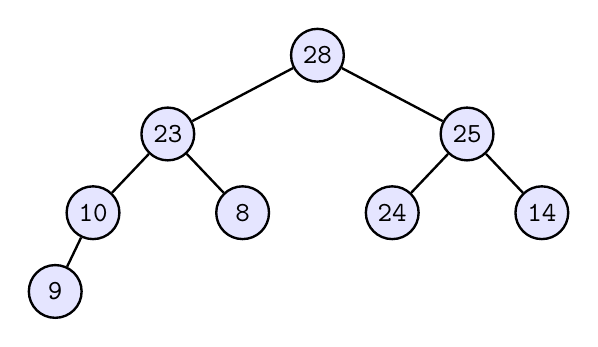
\begin{tikzpicture}

\fill[blue!10] (0.0, 0.0) circle (0.35);
\node [line width=0.03cm,black,minimum size=0.6699999999999999cm,draw,circle] at (0.0,0.0)(28){};\draw (0.0, 0.0) node[color=black] {\texttt{28}};
\fill[blue!10] (-1.9, -1.0) circle (0.35);
\node [line width=0.03cm,black,minimum size=0.6699999999999999cm,draw,circle] at (-1.9,-1.0)(23){};\draw (-1.9, -1.0) node[color=black] {\texttt{23}};
\fill[blue!10] (1.9, -1.0) circle (0.35);
\node [line width=0.03cm,black,minimum size=0.6699999999999999cm,draw,circle] at (1.9,-1.0)(25){};\draw (1.9, -1.0) node[color=black] {\texttt{25}};
\fill[blue!10] (-2.85, -2.0) circle (0.35);
\node [line width=0.03cm,black,minimum size=0.6699999999999999cm,draw,circle] at (-2.85,-2.0)(10){};\draw (-2.85, -2.0) node[color=black] {\texttt{10}};
\fill[blue!10] (-0.95, -2.0) circle (0.35);
\node [line width=0.03cm,black,minimum size=0.6699999999999999cm,draw,circle] at (-0.95,-2.0)(8){};\draw (-0.95, -2.0) node[color=black] {\texttt{8}};
\fill[blue!10] (0.95, -2.0) circle (0.35);
\node [line width=0.03cm,black,minimum size=0.6699999999999999cm,draw,circle] at (0.95,-2.0)(24){};\draw (0.95, -2.0) node[color=black] {\texttt{24}};
\fill[blue!10] (2.85, -2.0) circle (0.35);
\node [line width=0.03cm,black,minimum size=0.6699999999999999cm,draw,circle] at (2.85,-2.0)(14){};\draw (2.85, -2.0) node[color=black] {\texttt{14}};
\fill[blue!10] (-3.33, -3.0) circle (0.35);
\node [line width=0.03cm,black,minimum size=0.6699999999999999cm,draw,circle] at (-3.33,-3.0)(9){};\draw (-3.33, -3.0) node[color=black] {\texttt{9}};\draw[line width=0.03cm,black] (28) to  (23);
\draw[line width=0.03cm,black] (28) to  (25);
\draw[line width=0.03cm,black] (23) to  (10);
\draw[line width=0.03cm,black] (23) to  (8);
\draw[line width=0.03cm,black] (25) to  (24);
\draw[line width=0.03cm,black] (25) to  (14);
\draw[line width=0.03cm,black] (10) to  (9);
\end{tikzpicture}

\end{center}



where \verb!99! is a fake value, i.e.,
it's 
should not be considered part of the values in
the heap container.

Of course if two heaps have very different
heights, then you won't
be able to achieve
$O(\lg n)$ runtimes for insert and delete.
For instance if the second heap from the above
has only 4 values
(i.e., \verb!16!, \verb!13!, \verb!7!, \verb!3!),
then the resulting
merged heap (using the above method)
would look like this:

\begin{center}
\begin{tikzpicture}

\fill[white] (0.0, 0.0) circle (0.3);
\node [line width=0.03cm,black,minimum size=0.57cm,draw,circle] at (0.0,0.0)(10){};\draw (0.0, 0.0) node[color=black] {\texttt{10}};
\fill[white] (-3.0, -1.0) circle (0.3);
\node [line width=0.03cm,black,minimum size=0.57cm,draw,circle] at (-3.0,-1.0)(5){};\draw (-3.0, -1.0) node[color=black] {\texttt{5}};
\fill[white] (3.0, -1.0) circle (0.3);
\node [line width=0.03cm,black,minimum size=0.57cm,draw,circle] at (3.0,-1.0)(18){};\draw (3.0, -1.0) node[color=black] {\texttt{18}};
\fill[white] (-4.5, -2.0) circle (0.3);
\node [line width=0.03cm,black,minimum size=0.57cm,draw,circle] at (-4.5,-2.0)(0){};\draw (-4.5, -2.0) node[color=black] {\texttt{0}};
\fill[white] (-1.5, -2.0) circle (0.3);
\node [line width=0.03cm,black,minimum size=0.57cm,draw,circle] at (-1.5,-2.0)(7){};\draw (-1.5, -2.0) node[color=black] {\texttt{7}};
\fill[white] (-2.25, -3.0) circle (0.3);
\node [line width=0.03cm,black,minimum size=0.57cm,draw,circle] at (-2.25,-3.0)(6){};\draw (-2.25, -3.0) node[color=black] {\texttt{6}};
\fill[white] (-0.75, -3.0) circle (0.3);
\node [line width=0.03cm,black,minimum size=0.57cm,draw,circle] at (-0.75,-3.0)(8){};\draw (-0.75, -3.0) node[color=black] {\texttt{8}};\draw[line width=0.1cm,red,->,>=triangle 60] (10) to  (5);
\draw[line width=0.03cm,black,->,>=triangle 60] (10) to  (18);
\draw[line width=0.03cm,black,->,>=triangle 60] (5) to  (0);
\draw[line width=0.1cm,red,->,>=triangle 60] (5) to  (7);
\draw[line width=0.03cm,black,->,>=triangle 60] (7) to  (6);
\draw[line width=0.03cm,black,->,>=triangle 60] (7) to  (8);
\end{tikzpicture}

\end{center}


